\documentclass[runningheads]{llncs}
\usepackage[T1]{fontenc}
\usepackage[utf8]{inputenc}
\usepackage{amsmath,amssymb}
\usepackage{graphicx}
\usepackage{booktabs}
\usepackage{multirow}
\usepackage[hidelinks,pdfauthor={},pdftitle={}]{hyperref}

\emergencystretch=1em
\begin{document}

\title{Depth or Shots? The Number of QAOA Layers in Quantum Neighborhood
Search for the Permutation Flow Shop Problem}
\titlerunning{Depth or Shots?}
\author{Anonymous}
\institute{Anonymous}
\maketitle

\begin{abstract}
Quantum neighborhood search selects a scheduling move by sampling a QAOA
circuit and keeping the lowest-energy sample. Earlier gate-based neighborhood
studies of the permutation flow shop problem used one QAOA layer, and how
many layers such a neighborhood needs is open. We vary the depth $p$ from 1
to 10 in four neighborhoods (Adjacent, Fibonacci, Dynasearch and Motzkin)
with fixed angles calibrated on three kinds of training windows. We measure
the probability of sampling the optimal move and the
makespan of iterated local search on Taillard instances with 20 jobs. Without noise, $p = 1$ is worse than uniform sampling
in two neighborhoods. At $p = 2$ the best of 4096 samples is optimal in
almost every window of Dynasearch and Motzkin, and with 256 shots the median
deviation from the lower bound falls from 24\% under uniform sampling
to 15\%, below one layer with 4096 shots. In Adjacent and Fibonacci no depth
significantly improves the makespan over uniform sampling. On a simulated
16-qubit star processor with calibrated gate noise the hit rate of
Dynasearch and Motzkin peaks at $p = 2$. Every further layer adds about 150
CZ gates and pushes it back toward uniform sampling. On the real processor,
$p = 1$ does no better than uniform sampling, two layers bring no gain, and
three make Dynasearch significantly worse.
Beyond two layers the source of the angles matters more than the depth, and
the mean energy
minimized in calibration is a poor proxy for hitting the optimum.
\keywords{QAOA \and circuit depth \and flow shop \and neighborhood search \and fixed angles}
\end{abstract}

\section{Introduction}

The permutation flow shop problem (PFSP) asks for an order of $n$ jobs that
pass through $m$ machines so that the last job finishes as early as possible,
and the Taillard instances~\cite{taillard1993} remain its standard benchmark.
Iterated local search~\cite{lourenco2003} solves it well when the
neighborhood is large. Exponential neighborhoods, such as the Fibonacci
neighborhood of Bo\.{z}ejko et al.~\cite{bozejko2026new} and the Motzkin
neighborhood of Wojew\'{o}dzki and
Bo\.{z}ejko~\cite{wojewodzki2026soco,wojewodzki2025exit}, contain far more
moves than can be listed. The best move is then found by solving an
optimization problem, either by dynamic programming or by hybrid
evaluation~\cite{wojewodzki2026icaisc}.

Selecting the best combination of swaps can be written as a quadratic
unconstrained binary optimization (QUBO) problem~\cite{lucas2014ising}, so
the move can be sampled on quantum hardware. On quantum annealers these neighborhoods have been evaluated inside
iterated local search and simulated annealing~\cite{wojewodzki2026bpasts},
and a windowed QUBO decomposition extends the approach to instances with up
to 500 jobs~\cite{wojewodzki2026windowed}. On gate-based processors the same
QUBO is sampled with the quantum approximate optimization algorithm
(QAOA)~\cite{farhi2014qaoa}. Bo\.{z}ejko et
al.~\cite{bozejko2024cinti} applied hybrid quantum approximate algorithms to
the flow shop problem, and fixed-angle QAOA with windowed neighborhoods has
been run on IBM and IQM processors~\cite{wojewodzki2026gcmm,wojewodzki2026aciids}.
In this setting local search does not need the expected energy of the QAOA
state. It needs one good sample, the lowest-energy assignment among $S$
shots.

The gate-based neighborhood studies cited above used a single QAOA layer.
Most of the literature on depth deals with MaxCut and the Sherrington--Kirkpatrick
model~\cite{zhou2020,basso2022,wurtz2021fixed} and measures the expected cost
rather than the best of a finite sample inside a search loop.
Dudkiewicz~\cite{dudkiewicz2026depth} varied the depth for the
multidimensional knapsack problem, with angles optimized by COBYLA and a
different quality measure. It is therefore open whether a scheduling
neighborhood profits from deeper circuits, and whether noise leaves any room
for them.

This paper studies the depth $p$ of fixed-angle QAOA in four PFSP
neighborhoods. We calibrate angles for $p = 1, \dots, 10$ on three kinds of
training windows and measure, without noise, how often the circuit samples
the optimal move of the windows that local search builds. We then ask whether
more layers or more shots are the better use of a fixed search time and determine
the best depth under a gate noise model calibrated on a 16-qubit star
processor. We also measure the makespan of iterated
local search on Taillard instances with 20 jobs, with uniform sampling
($p = 0$) and the classical neighborhood search as references. Finally, we
run ILS on the IQM Sirius processor at $p = 2$ and $p = 3$ and compare these
runs with the $p = 1$ runs of an earlier campaign~\cite{wojewodzki2026aciids}.

\section{Related Work}

Farhi et al.~\cite{farhi2014qaoa} introduced QAOA, which alternates $p$ layers of a cost and a
mixer Hamiltonian and approaches adiabatic evolution as $p$ grows. Zhou et
al.~\cite{zhou2020} showed that optimal angles change smoothly with $p$ and
proposed the INTERP rule, which builds a depth-$(p+1)$ schedule by
interpolating the depth-$p$ one. Basso et al.~\cite{basso2022} evaluated
QAOA at depths far beyond $p = 1$ on large-girth regular graphs, and Wurtz
and Lykov~\cite{wurtz2021fixed} proposed fixed angles for regular MaxCut
graphs that need no optimization per instance. Galda et
al.~\cite{galda2021} showed that optimal angles transfer between random
graphs, which fixed angles rely on, and Akshay et al.~\cite{akshay2020} found
that a higher density of constraints raises the depth QAOA needs. Barkoutsos
et al.~\cite{barkoutsos2020cvar} replaced the expected cost of the QAOA state
by its conditional value at risk (CVaR), the mean over the best fraction of
the samples, which comes closer to the lowest-energy readout used here.
Mixers that keep the state inside the feasible set~\cite{hadfield2019} would
remove the penalty term at the cost of extra two-qubit gates in every layer,
so we keep the standard transverse-field mixer. QAOA and other variational algorithms have also been
applied to job shop scheduling~\cite{kurowski2023,amaro2022}, where the
circuit encodes a whole schedule rather than one move.

Noise limits how deep a useful circuit can be. Stilck Fran\c{c}a and
Garc\'{i}a-Patr\'{o}n~\cite{franca2021} showed that on noisy quantum processors the
output of variational algorithms approaches a state that efficient classical
methods can match once the circuit is deep enough. Harrigan et
al.~\cite{harrigan2021} ran QAOA on a superconducting processor and found
that for problems whose graph does not match the chip, routing adds gates and
the performance drops with problem size. Gnatowski et
al.~\cite{gnatowski2026routing} gave an exact routing algorithm for the star
topology of the processor used here.

\section{Quantum Neighborhood Search}

In the PFSP, $n$ jobs pass through $m$
machines in the same order, and a permutation $\pi$ fixes the order of the
jobs on every machine. The goal is to minimize the makespan
$C_{\max}(\pi)$, the time at which the last machine finishes the last job.
Iterated local search (ILS)~\cite{lourenco2003} applies the move that the
neighborhood $N(\pi)$ returns, even a worse one, and keeps the best
permutation found. A move stays tabu for the next nine iterations unless it
improves the best makespan. When the returned move is tabu, ILS applies a
double-bridge kick to one of the last ten best-so-far permutations, taken in
turn.

A move in the neighborhoods studied here is a set of disjoint swaps. Each
candidate swap $k$ has a precomputed makespan change $\Delta_k$, and a binary
variable $x_k$ selects it. The swap-selection QUBO~\cite{lucas2014ising}
\begin{equation}
  E(x) = \sum_k \Delta_k x_k + P \sum_{(k,l) \in \mathcal{C}} x_k x_l ,
  \qquad P = 1 + \sum_k |\Delta_k| ,
\end{equation}
sums the changes of the selected swaps and penalizes every pair in the
conflict set $\mathcal{C}$, so any assignment that breaks a constraint costs
more than doing nothing. The sum is exact for one swap and only approximates
the makespan change when selected swaps interact. We call the minimizer of
$E$ the optimal move. Table~\ref{tab:neigh} lists the four neighborhoods.
Adjacent selects exactly one swap of neighbors and uses the one-hot QUBO
\begin{equation}
  E(x) = \sum_i (\Delta_i - P)\,x_i + 2P \sum_{i<j} x_i x_j ,
  \qquad P = 2\max_i|\Delta_i| + 1 .
\end{equation}
Fibonacci~\cite{bozejko2026new} allows any set of disjoint adjacent swaps,
which gives a tridiagonal QUBO. Dynasearch~\cite{congram2002} and
Motzkin~\cite{wojewodzki2026soco} swap the end points of intervals and give
a QUBO with pairwise conflicts. Dynasearch forbids overlapping intervals,
while Motzkin also allows nested ones. We call Adjacent and Fibonacci the
\emph{linear} neighborhoods, since they swap only neighboring jobs, and
Dynasearch and Motzkin the \emph{dense} ones, since they swap any two positions.

\begin{table}[t]
\caption{The four neighborhoods ($F_{n+1}$, $M_n$: Fibonacci and Motzkin
numbers; last column: variables per window in ILS, $n = 20$).}
\label{tab:neigh}
\centering
\begin{tabular}{lllll}
\toprule
Neighborhood & Move & Moves & QUBO & Variables \\
\midrule
Adjacent   & one adjacent swap              & $n - 1$    & one-hot     & 1--16 (median 10) \\
Fibonacci  & disjoint adjacent swaps        & $F_{n+1}$  & tridiagonal & 1--16 (median 10) \\
Dynasearch & disjoint interval end swaps    & $2^{n-1}$  & pairwise    & 4--15 (median 14) \\
Motzkin    & non-crossing interval end swaps & $M_n$     & pairwise    & 4--15 (median 14) \\
\bottomrule
\end{tabular}
\end{table}

A whole permutation of $n = 20$ jobs gives more variables than a 16-qubit
processor can hold, so ILS splits the permutation into overlapping windows of
$w$ positions with overlap $0.5$ and solves one QUBO per
window~\cite{wojewodzki2026windowed,wojewodzki2026aciids}. Each window spans
$w = 17$ positions in the linear neighborhoods and $w = 6$ in the dense ones.
ILS drops candidates with a block filter in the spirit of Nowicki and
Smutnicki~\cite{nowicki1996} that uses the blocks of the last machine, the
runs of jobs it processes back to back. An adjacent swap is dropped when
neither of its jobs starts a block, and an interval swap when no job of its
span starts one. The filter is a heuristic and can drop an improving swap,
and it gives the window sizes in Table~\ref{tab:neigh}. In Adjacent, ILS
applies the window proposal with the lowest $\Delta$. In the other
neighborhoods a greedy pass goes over the selected swaps of all windows from
left to right and drops every swap that conflicts with one kept before it,
which also repairs an infeasible readout. ILS then applies the swaps that
remain. If no window selects a swap in Dynasearch or Motzkin, ILS applies
the best improving interval swap of the whole permutation, found
classically.

\section{QAOA at Depth $p$}

The substitution $x_k = (1 - Z_k)/2$ turns $E(x)$ into the Ising Hamiltonian
\begin{equation}
  H_C = \sum_k h_k Z_k + \sum_{k<l} J_{kl} Z_k Z_l ,
\end{equation}
which we scale so that its
largest coefficient has magnitude one. The depth-$p$ QAOA state is
\begin{equation}
  |\gamma,\beta\rangle = \prod_{\ell=1}^{p}
  e^{-i\beta_\ell H_M} e^{-i\gamma_\ell H_C} \, |{+}\rangle^{\otimes K},
  \qquad H_M = \sum_k X_k ,
\end{equation}
where $K$ is the number of variables in the window, and each layer costs one
$R_{ZZ}$ gate per coupling and one $R_Z$ and one
$R_X$ gate per qubit.

The angles are fixed in advance, so each window needs a single circuit
execution per move. For each neighborhood and each depth we calibrate one
schedule of angles $(\gamma_1, \dots, \gamma_p, \beta_1, \dots, \beta_p)$ by
minimizing
the mean of
\begin{equation}
  \frac{\langle H_C \rangle}{\sum_k |h_k| + \sum_{k<l} |J_{kl}|}
\end{equation}
over a
training set of windows from three of the test instances~\cite{taillard1993}.
These instances supply a tenth of the windows of the window study and three
of the 12 instances used with noise. At $p = 1$ the best
point of a $25 \times 13$ grid over $\gamma \in [0, \pi]$ and
$\beta \in [0, \pi/2]$ gives the angles. For $p \ge 2$ Nelder--Mead starts
from four schedules: the depth-$(p-1)$ schedule with an empty last layer,
which keeps the objective from rising, its INTERP resample~\cite{zhou2020}
and two copies of the resample with Gaussian noise of standard deviation
0.15. Each run takes at most $400p$ iterations, and the best of the four
results is kept.

We build three angle tables that differ only in the training windows. The
\emph{small-window} table uses windows of $w = 6$ positions and goes up to
$p = 10$. In the dense neighborhoods these windows keep only the improving
swaps ($\Delta_k < 0$). The \emph{big-window} table uses windows of the ILS
sizes without the $\Delta$ filter, in the linear neighborhoods also without
the block filter, and the \emph{ILS-window} table uses windows captured from
ILS itself. Both go up to $p = 5$. For the dense neighborhoods the last two
coincide and differ from the small-window table only in the $\Delta$ filter.

ILS samples the circuit $S$ times and selects the sample with the lowest
original QUBO energy. If $P_{\mathrm{opt}}$ is the probability of an optimal
assignment, the best of $S$ samples is optimal with probability
\begin{equation}
  1 - (1 - P_{\mathrm{opt}})^S ,
\end{equation}
which we call the hit rate, so more shots
can make up for a weaker distribution.

On the star-shaped processor every qubit couples only to a central
resonator, and a two-qubit interaction first moves one qubit's state into the
resonator. One $R_{ZZ}$ gate then compiles to two CZ gates and about two
MOVE gates~\cite{gnatowski2026routing}. A dense window of 15 variables needs
150 (Motzkin) to 180 (Dynasearch) CZ gates per layer, and the cost grows in
proportion to $p$.
Table~\ref{tab:e3} compares the star with a 20-qubit square lattice (IQM
Apollo), where routing inserts SWAP gates; both use the IQM transpiler at
optimization level~1.

\section{Experimental Setup}

The noiseless experiments use the 30 Taillard instances with $n = 20$ jobs,
ten for each number of machines $m \in \{5, 10, 20\}$~\cite{taillard1993}, and
the noisy and hardware experiments use the first four of each group, 12
instances in all. ILS starts from the identity permutation, as in the earlier
campaign~\cite{wojewodzki2026aciids}. We evaluate QAOA at three levels. On the
noiseless level the circuit is sampled from its exact statevector. On the
noisy level a simulated 16-qubit star processor reproduces the gate
fidelities and readout errors that IQM reported for the Sirius quantum processor on
23~October~2026. In its default \emph{calibrated} mode a depolarizing channel
gives every single-qubit and CZ gate exactly the measured fidelity, and a
\emph{thermal} mode adds $T_1$/$T_2$ relaxation. We run the thermal mode only on the first
instance of each group at $p = 1$, 3 and 6 (Adjacent: 1 and 3, since its
big-window table ends at $p = 5$). Neither mode applies noise to the MOVE
gates or to idle qubits, although a MOVE gate has a measured error of about
1\% and a dense layer holds about as many MOVE as CZ gates, so the
calibrated mode is optimistic for deep circuits. On the hardware level the
circuits run on Sirius itself.

The window study reads the QAOA distribution of single windows. We capture
the windows of the first ILS move from the identity and from two random
permutations of every instance, 1440 windows in total, and compute their
optimum by enumeration. In 1195 of them the optimal energy is negative. The
noiseless level gives $P_{\mathrm{opt}}$ exactly for $p = 0, \dots, 10$. The
noisy level takes the 161 windows with negative optimal energy from the first
ILS move from the identity on the 12 instances (57 in each dense
neighborhood, 24 in Adjacent and 23 in Fibonacci) and samples each once with
4096 shots for $p = 0, \dots, 6$.

The ILS study measures the makespan. Without noise, ILS runs for 10~s of wall
time in four variants: QAOA with the small-window table for
$p = 1, \dots, 10$, QAOA with the big-window table for Adjacent and the
ILS-window table for Fibonacci ($p \le 5$), uniform sampling ($p = 0$) with
the same lowest-energy readout, and the classical search. The classical
search chooses the move from the whole permutation without windows, by
computing the makespan of every swap in Adjacent and by dynamic programming
over the same swap changes $\Delta_k$ in the other neighborhoods. The 10~s
include simulating and sampling every circuit, with eight runs in parallel on
one computer. The QAOA variants use $S = 256$ and $S = 4096$ shots. ILS runs
once per instance in the linear neighborhoods and five times in the dense
ones. A noisy
simulator needs minutes per circuit, so its wall time says nothing about the
quantum processor; each noisy run therefore makes exactly as many moves as Sirius made
in 10~s on the same instance at $p = 1$~\cite{wojewodzki2026aciids}. On the
quantum processor, ILS repeats that campaign at $p = 2$ and $p = 3$, once per instance,
with the small-window table and, for Adjacent, the big-window table. The calibration of the quantum processor on the day of these runs (6~November~2026) was
close to the one the simulator uses, with a median CZ error of 1.9\% against
1.7\%. The runs at $p = 1$ are a month older and come from a different
calibration. ILS checks the 10~s budget only between moves, so on Sirius a
dense run makes a single move, which ends 12 to 17~s after the start, and a
linear run makes one to three.

We measure quality by the deviation from the Taillard lower bound $LB$ in
percent,
\begin{equation}
  \mathrm{PRD} = 100\,\frac{C_{\max} - LB}{LB} ,
\end{equation}
average it over the runs of an instance and take the median over instances.
We compare two settings with a two-sided paired sign test over instances,
which ignores ties, and call a difference significant at the 5\% level
without correcting for the number of comparisons. The upper bounds reported for these
instances~\cite{taillard1993} lie 1 to 26\% above $LB$ (median 8\%), so a PRD
of about 9\% is already close to them.

\section{Results}

Without noise one layer is not enough (Fig.~\ref{fig:e1}). With the
small-window table, which ILS uses, only Adjacent samples the optimal move
clearly more often than uniform sampling at $p = 1$. Motzkin barely beats it,
and Fibonacci and Dynasearch fall below it. From
$p = 2$ this table samples the optimum of a dense window about a hundred
times more often than uniform sampling, and with 4096 shots the best sample
is then almost always optimal (Fig.~\ref{fig:hits}). Further layers therefore
add little, and shots can take their place. The gain is not monotone in $p$,
and the best angle table depends on the neighborhood. In Dynasearch the
ILS-window table reaches a far lower mean energy on the ILS windows than the
small-window table, yet at $p = 2$ it samples their optimum only about a
tenth as often, and Motzkin shows the same from $p = 3$.

In Table~\ref{tab:e3} the square lattice needs about twice as many CZ gates
as the star in the dense windows. With noise this cost decides the best depth
(Fig.~\ref{fig:e4}). In the dense neighborhoods the best sample is optimal
most often at $p = 2$, clearly so in Motzkin, while in Dynasearch $p = 3$ and
$p = 4$ miss only two or three more windows. At $p = 6$ the circuit is no
better than uniform sampling. In the linear neighborhoods uniform sampling
already finds the optimum in about nine of ten windows, and no depth beats it
by more than a few windows.

The same picture appears in the makespan of ILS (Table~\ref{tab:e5}). With
256 shots, $p = 2$ lowers the median PRD in the dense neighborhoods from
about 24\% under uniform sampling to 15\% and beats uniform sampling on every
instance. With 4096 shots it still wins on almost all of them. Two layers
with 256 shots also beat one layer with 4096 shots on almost every instance,
while at $p = 2$ the extra shots bring no gain. Deeper circuits lose because
each simulated move takes longer and fewer moves fit into 10~s
(Fig.~\ref{fig:moves}); after the same number of moves they do about as well
as $p = 2$. In the linear neighborhoods no depth beats uniform sampling with
either angle table, and several depths lose to it significantly, since deeper
circuits make fewer moves. In every neighborhood the classical search, which works on the
whole permutation and makes tens to hundreds of times more moves in 10~s,
stays better than all QAOA variants. Since at $p = 2$ the best sample is
almost always the window optimum, this gap comes mainly from the windows and
the number of moves, not from the sampler.

Because every dense run in Table~\ref{tab:hw} makes a single move from the
identity, these rows judge the windows of Fig.~\ref{fig:e4} by the makespan.
The identity itself lies at a median PRD of 40\%, so the table shows what one
to three moves achieve and cannot be compared with Table~\ref{tab:e5}. On the noisy simulator
Dynasearch at $p = 2$ beats $p = 1$ on almost every instance. On Sirius, Dynasearch at $p = 1$ does about as well as uniform
sampling. The gain of $p = 2$ does not survive on Sirius. In the
linear neighborhoods two and three layers leave the median PRD almost
unchanged. In the dense ones the second layer brings no gain and the third
makes the median worse. Dynasearch at $p = 3$ is significantly worse than
uniform sampling ($p = 0$) and than the simulator at the same depth. It also
loses significantly to the quantum processor at $p = 1$, whose runs used another
calibration, and, though not significantly, to $p = 2$ from the same day. At
$p = 1$ the quantum processor does better than the model, at $p = 2$ the two are level,
and at $p = 3$ the model overrates the quantum processor. The median of Motzkin
rises with each layer, although none of its sign tests is significant.

\begin{figure}[t]
\centering
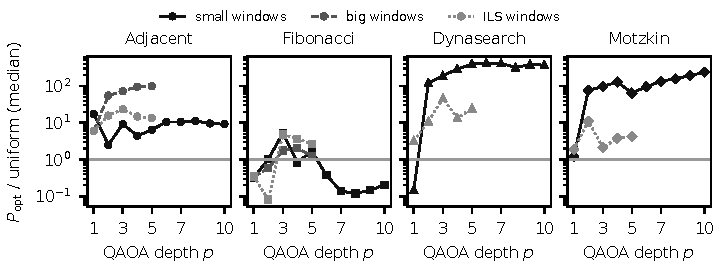
\includegraphics[width=\textwidth]{figures/fig1_e1_en.pdf}
\caption{$P_{\mathrm{opt}}$ relative to uniform sampling versus $p$ for the
three angle tables (median over windows with negative optimal energy;
noiseless).}
\label{fig:e1}
\end{figure}

\begin{figure}[t]
\centering
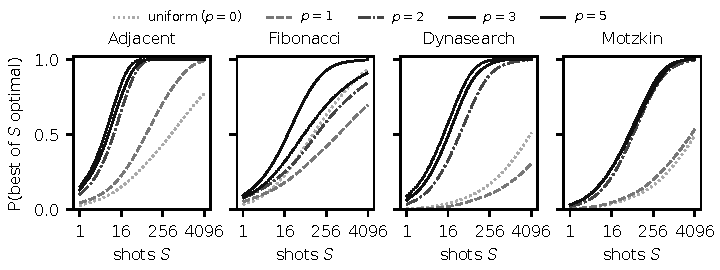
\includegraphics[width=\textwidth]{figures/fig2_hits_en.pdf}
\caption{Probability that the best of $S$ samples is optimal versus $S$
(noiseless; Adjacent: big-window table, others: small-window table).}
\label{fig:hits}
\end{figure}

\begin{table}[t]
\caption{CZ gates per window after compilation for the star of Sirius and a
square lattice (median over the first-move windows of each neighborhood on
the 12 instances).}
\label{tab:e3}
\centering
\begin{tabular}{lrrrrrrrr}
\toprule
 & \multicolumn{2}{c}{$p = 1$} & \multicolumn{2}{c}{$p = 3$} & \multicolumn{2}{c}{$p = 6$} & \multicolumn{2}{c}{$p = 10$} \\
\cmidrule(lr){2-3}\cmidrule(lr){4-5}\cmidrule(lr){6-7}\cmidrule(lr){8-9}
Neighborhood & star & lattice & star & lattice & star & lattice & star & lattice \\
\midrule
\csname @@input\endcsname tables/tab1_e3.tex 
\bottomrule
\end{tabular}
\end{table}

\begin{figure}[t]
\centering
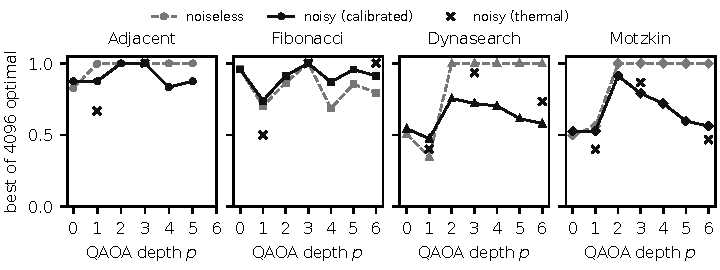
\includegraphics[width=\textwidth]{figures/fig3_noise_en.pdf}
\caption{Share of windows in which the best of 4096 samples is optimal
versus $p$ (12 instances; thermal noise: first instance of each group; angle
tables as in Fig.~\ref{fig:hits}).}
\label{fig:e4}
\end{figure}

\begin{table}[t]
\caption{ILS without noise, 10~s: median PRD [\%] over 30 instances
(small-window table; classical: search over the whole permutation).}
\label{tab:e5}
\centering
\begin{tabular}{llrrrrrrr}
\toprule
Neighborhood & $S$ & $p=0$ & $p=1$ & $p=2$ & $p=3$ & $p=6$ & $p=10$ & classical \\
\midrule
\csname @@input\endcsname tables/tab2_prd.tex 
\bottomrule
\end{tabular}
\end{table}

\begin{table}[t]
\caption{Median PRD [\%] on the 12 instances with $S = 4096$ (simulated rows:
small-window table and the moves Sirius made at $p = 1$; Adjacent on Sirius at
$p \ge 2$: big-window table; --: not run).}
\label{tab:hw}
\centering
\begin{tabular}{llrrrrr}
\toprule
Neighborhood & level & $p=0$ & $p=1$ & $p=2$ & $p=3$ & $p=6$ \\
\midrule
\csname @@input\endcsname tables/tab3_hw_en.tex 
\bottomrule
\end{tabular}
\end{table}

\begin{figure}[t]
\centering
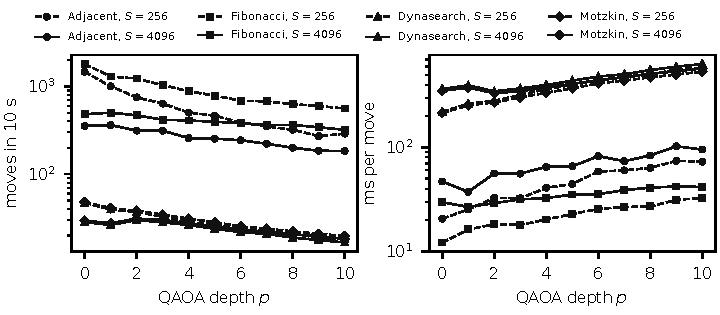
\includegraphics[width=\textwidth]{figures/fig4_moves_en.pdf}
\caption{Moves in 10~s and time per move versus $p$ (noiseless; $p = 0$:
uniform sampling).}
\label{fig:moves}
\end{figure}

\section{Discussion and Conclusions}

Without noise, a single QAOA layer with fixed angles is too weak for the
dense neighborhoods, while two layers find the optimal move in almost every
dense window. With simulated noise $p = 2$ also gives the highest hit rate,
because every further layer costs about 150 CZ gates. In the linear
neighborhoods a window holds so few variables that uniform sampling already
finds most optima, and ILS does at least as well with it as with QAOA.
In simulation the answer to the title question is therefore depth up to two
layers, and without noise shots beyond them, since in the dense neighborhoods the second
layer is worth more than sixteen times as many shots. On Sirius, however,
extra layers do not help, and even one layer does no better than uniform
sampling. The gain from depth seen in simulation does not carry over to this
quantum processor. Beyond two layers the angles matter more than the depth, and
calibrating them for the mean energy does not target the best sample, which
is all that local search uses.

The study covers only 20 jobs and fixed angles, it
compares depth with shots only without noise, and the window energy is exact
only when the swaps do not interact. Windows of up to 16 variables are also
easy to enumerate classically. In the dense neighborhoods the classical
fallback produced none of the single moves of the noisy simulator and at
most one of those on Sirius, so it does not drive the results under noise.
The missing noise on idle qubits and MOVE gates may explain why Sirius seemed
noisier than the simulator and why extra layers hurt more on the quantum processor,
since a dense circuit at $p = 3$ contains about 500 MOVE gates. Future work will
calibrate the angles for the hit rate, for
instance with the CVaR objective~\cite{barkoutsos2020cvar}, and choose the
depth per window.

\subsubsection{Use of AI Tools.} The authors used a large language model to
help draft and edit parts of the text, write the experiment scripts and
typeset the paper; the research, its results and their
interpretation are entirely the authors' own.

\bibliographystyle{splncs04}
\bibliography{references}

\end{document}
